\documentclass{beamer}

\input{header.tex}
\usepackage[font=footnotesize]{caption}

\usetheme{Warsaw}
\usecolortheme{beaver}

\setbeamertemplate{tableofcontents}[triangle]
\setbeamertemplate{itemize item}[triangle]
\setbeamertemplate{itemize subitem}[triangle]
\setbeamertemplate{footline}{
	\mbox{
		\begin{beamercolorbox}[wd=.5\paperwidth,ht=2.5ex,dp=1.125ex,leftskip=.3cm plus1fill,rightskip=.3cm]{author in head/foot}%
			\usebeamerfont{author in head/foot}\insertshortauthor
		\end{beamercolorbox}%
		\begin{beamercolorbox}[wd=.5\paperwidth,ht=2.5ex,dp=1.125ex,leftskip=.3cm,rightskip=.3cm plus1fil]{title in head/foot}%
			\usebeamerfont{title in head/foot}\insertshorttitle\hfill\insertframenumber/\inserttotalframenumber
	\end{beamercolorbox}}%
	\vskip0pt%
}


\author{Lino Lemmer}
\title[Brustkrebsdiagnose durch Ultraschall und MRT]{Brustkrebsdiagnose durch ultraschallinduzierte Gewebeverschiebung}
\institute{HISKP - Uni Bonn}
\subtitle{Stand Bachelorarbeit}

\date{30. Januar 2015}

\begin{document}

%Folie 1

	\begin{frame}
		\titlepage
	\end{frame}

    \section{Einleitung}

%Folie 2

	\begin{frame}
		\frametitle{Motivation}

        \begin{itemize}
            \item
                über \num{75000} Brustkrebs-Neuerkrankungen allein 2014
            \item
                Nachteile bei gängigen Diagnoseverfahren:
                \begin{itemize}
                    \item
                        manuelle Palpation: Tumore im Frühstadium und
                        tiefliegende Tumore schwer zu finden
                    \item
                        Mammographie: körperliche Belastung durch
                        Röntgenstrahlung
                    \item
                        DCE-MRT: körperliche Belastung durch Kontrastmittel
                    \item
                        psychische Belastung durch falsch-positiv Diagnose
                \end{itemize}
        \end{itemize}
	\end{frame}

%Folie 3

		\begin{frame}
			\frametitle{Kombination von Ultraschall und MRT}
            \begin{itemize}
                \item
                    gleicher Ansatz wie Palpation: Sichtbarmachen der Veränderung elastischer
                    Eigenschaften des Gewebes durch Kombination von Ultraschall
                    und MRT
                \item
                    Schalldruck $\to$ Gewebeverschiebung abhängig von
                    Elastizität des Gewebes
                \item
                    Aufnahme der Verschiebung durch Phasenbilder im MRT
                \item
                    Vorteile:
                \begin{itemize}
                    \item 
                        keine körperliche Belastung durch Strahlung
                    \item
                        größere Eindringtiefe als manuelle Palpation
                    \item
                        unabhängig von Erfahrung des untersuchenden Arztes
                \end{itemize}
            \item
                Studie  an 10 Patientinnen soll zeigen ob Spezifität erhöht werden kann
            \end{itemize}
		\end{frame}

	\section{Messvorgang}

    \subsection{Gewebeverschiebung}
%Folie 4

    \begin{frame}
        \frametitle{Gewebeverschiebung durch Schallstrahlungsdruck}
        \begin{figure}
            \centering
            \includegraphics[width=.7\textwidth]{../Abbildungen/Verschiebung_Gewebe.pdf}
        \end{figure}
    \end{frame}

    \subsection{Sequenz}

%Folie 5

	\begin{frame}
		\frametitle{Sequenz}
        \begin{figure}
            \centering
            \includegraphics[width=.45\textwidth]{../Abbildungen/sediffmono.pdf}
        \end{figure}
	\end{frame}

    \subsection{Verschiebevorrichtung}


%Folie 6

	\begin{frame}
		\frametitle{Verschiebevorrichtung}
        \begin{itemize}
            \item 
                Aufnahme einer Schicht dauert über eine Minute
            \item
                Maximalzeit im MRT durch Ethikkommission begrenzt
            \item
                Patienten mit Läsion an bekannter Stelle
            \item
                Ultraschall soll schnell und zuverlässig an Ort der Läsion gefahren werden können $\to$ Verschiebevorrichtung
        \end{itemize}
	\end{frame}

%Folie 7

	\begin{frame}
		\frametitle{Verschiebevorrichtung}
        % Lage von Patient über Spiegel
        \begin{figure}
            \centering
            \begin{tikzpicture}
    % Wannen

    % groß
    \draw[thick] (-2.5,0) -- (-2.5,-2.7) 
        -- (4.5,-2.7) 
        -- (4.5,0);

    % klein
    \draw[thick] (1.8,.5) -- (1.8,-1);
    \draw[thick] (4.2,.5) -- (4.2,-1);
    \draw (1.8,-0.8) -- (4.2,-0.8);
    \draw[dashed] (4.0,-.8) -- (4.6,-1.2) node[right]{Mylarfolie};

    % Wasser
    \draw[wave, blue] (-2.5, -.2) -- (1.8,-.2);
    \draw[wave, blue] (4.2, -.2) -- (4.5,-.2);
    \draw[wave, blue] (1.8, .2) -- (2.37,.2);
    \draw[wave, blue] (3.67,.2) -- (4.2,.2);

    % Spiegel
    \draw[thick] (2.5, -2.5) 
        -- (3.5,-1.5) 
        -- (3.6,-1.6) 
        -- (2.6,-2.6) 
        -- (2.5,-2.5);
    \draw[dashed] (3.1,-2.0) -- (3.3,-2.9) node[below] {Spiegel};

    % Frau
    \draw[thick] (4.5,.8) 
        -- (4.3,.8) 
        to[in=0, out=180] (3.,-.5) 
        to[in=-10, out=180] (1.8, .8)
        to[in=10, out=170] (1.2,.8)
        to[in=10, out=190] (1.,.2)
        to[in=-0, out=170] (.45,.2)
        to[in=-10, out=180] (.35,.0)
        to[in=-10, out=170] (-.1,.2)
        to[in=-20,out=170] (-.5,.3)
        to[in=-90,out=160] (-.8,.8);

    % US-Emitter
    \draw[thick] (-1.9,-2.5) 
        -- (-2.1,-2.5) 
        -- (-2.1,-1.5) 
        -- (-1.9,-1.5) ;
    \draw[thick, bend right] (-1.9,-1.5) to (-1.9,-2.5);
    \draw[dashed] (-2.075,-2.0) -- (-2.7,-1.7) node[left]{\parbox{1.3cm}{US-\\Emitter}};

   % Ultraschall
    \draw (-1.92,-2.45) -- (2.9,-2.1) -- (3.0,.3);
    \draw (-1.92,-1.55) -- (3.2,-1.8) -- (3.0,.3);
\end{tikzpicture}

        \end{figure}
	\end{frame}

%Folie 8

	\begin{frame}
		\frametitle{Verschiebevorrichtung}
        \begin{figure}
            \centering
            \resizebox{\textwidth}{!}{
                % Tikzpicture Verschiebevorrichtung
    \begin{tikzpicture}
        % PC
        \draw (0,0) rectangle (1,1);
        \draw (-.2,-.2) rectangle (1.2,1.2);
        \draw (-.2,-.2) -- (-.4,-.4) -- (1.4,-.4) -- (1.2,-.2);
        \node at (.5,.5) {PC};

        % Kabel
        \draw[out=0, in=180]
            (1.2,.4) to (3,-.55)
            (1.2,.5) to (3,.45)
            (1.2,.6) to (3.,1.45);

        % Steuerbox mit Schrittmotoren
        \draw (3.,-1.1) rectangle (7,2);
        \foreach \y in {-1.0,0,1}
        \draw (3,\y) rectangle node{1} (4,\y+.9);

        % Kolben
        % Kolben 1
        \draw (4, -.7) rectangle (5.5,-.4);
        \draw[ultra thick] (4,-.55) -- (4.5,-.55);
        \draw (4.5,-.7) rectangle (4.6,-.4);

        % Kolben 2
        \draw (4, .3) rectangle (6.8,.6);
        \draw[ultra thick] (4,.45) -- (4.5,.45);
        \draw (4.5,.3) rectangle (4.6,.6);

        % Kolben 3
        \draw (4, 1.3) rectangle (5.,1.6);
        \draw[ultra thick] (4,1.45) -- (4.5,1.45);
        \draw (4.5,1.3) rectangle (4.6,1.6);

        % Verschiebevorrichtung
        \draw (8.7,-.2) rectangle (11.8,1.1);

        % Kolben 2
        \draw (8.8,.3) rectangle (11.6,.6);
        \draw[ultra thick] (9.4,.45) -- (12,.45);
        \draw (9.3,.3) rectangle (9.4,.6);

        % Kolben 1
        \draw (12,1.2) rectangle (12.3,-.3);
        \draw[ultra thick] (12.15,.6) -- (12.15,-.7);
        \draw (12,.7) rectangle (12.3,.6);

        % Kolben 3
        \draw (12.4,.9) rectangle (13.4,1.2);
        \draw[ultra thick] (13.0,1.05) -- (13.8,1.05);
        \draw (12.9,.9) rectangle (13.0,1.2);

        % Verbindung Kolben 1, 3 Emitter und Spiegel
        \draw (12.1,-.7) -- (12.4,-.7) -- (12.4,1.2);
        \draw (12.4,.5) -- (12.5,.5) coordinate (a) ;
        \draw (12.4,.8) --  (12.5,.8) coordinate (b);
        \draw[bend left] (b) to (a);
        \draw  ($(b)!.5!(a)$) -- (12.7,0) node[below]{4} ;
        \draw (13.8, 1.2) -- (13.8, 0.9);
        \draw (13.7,.9) rectangle coordinate (spiegel) (13.9,.4);
        \draw (spiegel) -- (13.5,0) node[below]{5};

        % Schläuche mit Steckverbindung und Kupplungen

        \draw[double] (5.4,-.4) to [out=90, in=-90] (6.9,.4) to [out=90, in=-90] (6.6,2) to [out=90, in=180] (7.6,2.6) -- (8.,2.6);
        \draw[ultra thick] (7.6,2.6) -- coordinate (S1)  (7.8,2.6) ;
        \draw (8.,2.5) rectangle coordinate (K1) (8.3,2.7);
        \draw[double] (8.3,2.6) -- (8.55,2.6);
        \draw[double] (8.65,2.6) to [out=0, in=90] (12.15,1.2);

        \draw[double] (6.6,.6) to [out=90, in=-90] (6.5,2) to [out=90, in=180] (7.6,2.3) -- (8.,2.3);
        \draw[ultra thick] (7.6,2.3) --  coordinate (S2) (7.8,2.3) ;
        \draw (8.,2.4) rectangle coordinate (K2) (8.3,2.2);
        \draw[double] (8.3,2.3) -- (8.51,2.3);
        \draw[double] (8.61,2.3) to [out=0, in=90] (9,.6);
        
        \draw[double] (4.9,1.6) to [out=90, in=-90] (6.4,2) to [out=90, in=180] (7.6,2.9) -- (8.,2.9);
        \draw[ultra thick] (7.6,2.9) -- coordinate (S3) (7.8,2.9);
        \draw (8.,2.8) rectangle coordinate (K3) (8.3,3.0);
        \draw[double] (8.3,2.9) -- (8.59,2.9);
        \draw[double] (8.69,2.9) to [out=0, in=90] (12.6,1.2);

        \draw (8.5,2.2) -- (8.6,3.0);
        \draw (8.6,2.2) -- (8.7,3.0);

        \node (S) at (7.5,3.8) {2};
        \foreach \y in {(S1), (S2), (S3)}
            \draw (S) -- \y;

        \node (K) at (8.3,3.8) {3};
        \foreach \y in {(K1), (K2), (K3)}
            \draw (K) -- \y;

        % Druckausgleich

            \draw (13.,-2) rectangle node {6} (13.75,-1);

            \draw[double] (12,-.2) to [out=180, in=180] (13,-1.3);
            \draw[double] (11.5,.3) to [out=-90, in=180] (13,-1.4); 
            \draw[double](13.3,.9) to [out=-90, in=180] (13,-1.2);

        % Beschriftung
        \node at (0,4) {\parbox{4.5cm}{
                1: Schrittmotor \\
                2: Steckverbindung \\
                3: Kupplung, tropffrei \\
                4: Ultraschallemitter \\
                5: Spiegel \\
                6: Druckausgleichsbehälter
            }
        };
    \end{tikzpicture}

            }
        \end{figure}
	\end{frame}

    \section{Verbesserung der Verschiebevorrichtung}

%Folie 9

	\begin{frame}
		\frametitle{Problem: Dichtungsringe}
        \begin{itemize}
            \item 
                nach längerem Stehen: Kolben sitzen fest
        \end{itemize}
		\begin{columns}
			\column{0.5\textwidth}
            vorher:
            \begin{figure}
                \centering
                \resizebox{.9\textwidth}{!}{% Tikzpicture Dichtungsring in schmaler Nut
        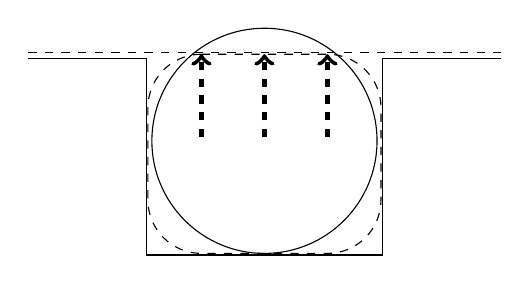
\begin{tikzpicture}
            \draw (.5,0) -- (2,0) -- (2,-2.5) -- (5,-2.5) -- (5,0) -- (6.5,0) ;
            \draw (3.5,-1.05) circle (1.43);
            \draw[dashed] (.5,.07) -- (6.5,.07);
            \foreach \x in {2.7, 3.5, 4.3} \draw[ultra thick, ->, dashed] (\x,-1) -- (\x,0.05);
            \draw[dashed] (2.7,.05) 
            -- (4.3,.05) 
            arc (90:0:.68) 
            -- (4.98,-1.8) 
            arc (0:-90:.68)
            -- (2.7,-2.48)
            arc (-90:-180:.68)
            -- (2.02,-.63)
            arc (-180:-270:.68);
        \end{tikzpicture}
}
            \end{figure}
            \begin{itemize}
                \item 
                    Nut etwa so breit wie Ring
                \item
                    zwei Ringe pro Kolben
                \item
                    Silikon-basiertes Schmiermittel
            \end{itemize}
			\column{0.5\textwidth}
            nachher:
            \begin{figure}
                \centering
                \resizebox{.9\textwidth}{!}{% Tikzpicture für Dichtungsring in breiter Nut
        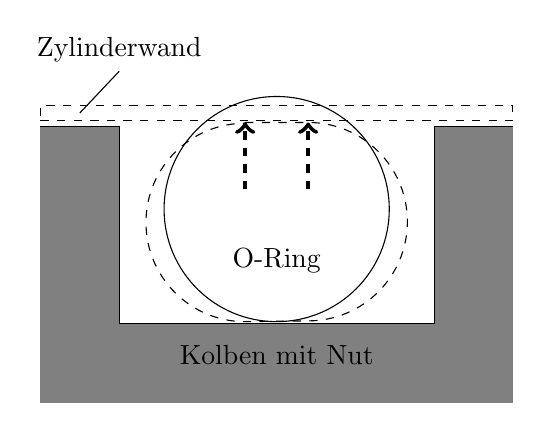
\begin{tikzpicture}
            \draw[gray, fill=gray] (1,0) -- (2,0) -- (2,-2.5) -- (6,-2.5) -- (6,0) -- (7,0) -- (7,-3.5) -- (1, -3.5) -- (1,0) ;
            \draw (1,0) -- (2,0) -- (2,-2.5) -- (6,-2.5) -- (6,0) -- (7,0) ;
            \draw (4,-1.05) circle (1.43);
            \draw[dashed] (1,0.07) -- (7,0.07) -- (7,.27) -- (1,.27) -- (1,.07) ;
            \foreach \x in {3.6, 4.4} \draw[ultra thick, ->, dashed] (\x,-.8) -- (\x,0.05);
            \draw[dashed] (3.6,.05) 
            -- (4.4,.05) 
            arc (90:-90:1.26) 
            -- (3.6,-2.48)
            arc (-90:-270:1.26);

            % Beschriftungen

            \draw (1.5,.17) -- (2.0,.7) node[above] {Zylinderwand};
            \node at (4.0,-2.9)  {Kolben mit Nut};
            \node at (4.0,-1.7) {O-Ring};
        \end{tikzpicture}
}
            \end{figure}
            \begin{itemize}
                \item 
                    breitere, tiefere Nut
                \item
                    ein Ring pro Kolben
                \item
                    PTFE-Spray als Schmiermittel
            \end{itemize}
		\end{columns}
	\end{frame}

%Folie 10

	\begin{frame}
		\frametitle{Ausblick/todo}
        \begin{itemize}
            \item 
                Steckverbindung zur Befüllung leiert Schläuche aus
                \begin{itemize}
                    \item
                        momentane Lösung: Abschneiden
                    \item 
                        Problem: endliche Schlauchlänge
                    \item
                        Plan:
                        \begin{figure}
                            \centering
                            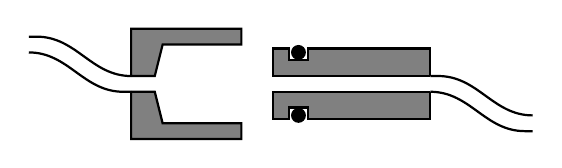
\begin{tikzpicture}
                                \draw[thick] (-1.1,.5) 
                                -- (-1,.5) 
                                to[in=180, out=0] (.2,.0);
                                \draw[thick, fill=gray] (.2,.0)
                                -- (.2,.6)
                                -- (1.6,.6)
                                -- (1.6,.4)
                                -- (.6,.4)
                                -- (.5,.0)
                                -- (.2,.0);

                                \draw[thick] (-1.1,.3) 
                                to[in=180, out=0] (.1,-.2)
                                -- (.2,-.2);
                                \draw[thick, fill=gray] (.2,-.2)
                                -- (.2,-.8)
                                -- (1.6,-.8)
                                -- (1.6,-.6)
                                -- (.6,-.6)
                                -- (.5,-.2)
                                -- (.2,-.2);

                                \draw[thick, fill=gray] (4,0)
                                -- (2,0)
                                -- (2,.35)
                                -- (2.2,.35)
                                -- (2.2,.2)
                                -- (2.45,.2)
                                -- (2.45,.35)
                                -- (4.,0.35)
                                -- (4.,0.);
                                \draw[thick] (4,0)
                                -- (4.1,0.)
                                to[in=180, out=0] (5.3,-.5);

                                \draw[thick,fill=gray] (4,-.2)
                                -- (2,-.2)
                                -- (2,-.55)
                                -- (2.2,-.55)
                                -- (2.2,-.4)
                                -- (2.45,-.4)
                                -- (2.45,-.55)
                                -- (4,-.55)
                                -- (4,-.2);
                                \draw[thick] (4,-.2)                        
                                to[in=180,out=0] (5.2,-.7)
                                -- (5.3,-.7);

                                \draw[thick, fill] (2.325,-.5) circle(.08);
                                \draw[thick, fill] (2.325,.3) circle(.08);


                            \end{tikzpicture}
                        \end{figure}
                \end{itemize}
            \item
                Eindringen von Luft bei Benutzung
        \end{itemize}
    \end{frame}

    \section{Erste Messung}

    \subsection{Bilder}

    % Folie 11

    \begin{frame}
        \frametitle{Erste Messung}
        \begin{itemize}
            \item 
                Probandin mit in MRT gut sichtbarem Fibroadenom (gutartiger Tumor)
                \begin{columns}
                    \column{.5\textwidth}
                    \begin{figure}
                        \centering
                        \includegraphics[width=.8\textwidth]{../Abbildungen/2014-11-27_9_7_amp.png}
                    \end{figure}
                    \column{.5\textwidth}
                    \begin{figure}
                        \centering
                        \includegraphics[width=.8\textwidth]{../Abbildungen/2014-11-27_19_1_phase.png}
                    \end{figure}
                \end{columns}
        \end{itemize}
    \end{frame}

    %Folie 12

    \begin{frame}
        \frametitle{Erste Messung}
        \begin{columns}
            \column{0.5\textwidth}
            Phasenbild nach unwrappen
            \begin{figure}
                \centering
                    \includegraphics[width=.9\linewidth]{../Abbildungen/standart_mask.pdf}
                \end{figure}
                \column{0.5\textwidth}
                Phasenbild ohne Untergrund
                \begin{figure}
                    \centering
                    \includegraphics[width=.9\linewidth]{../Abbildungen/diff_standart_mask.pdf}
                \end{figure}
            \end{columns}
	\end{frame}

    \subsection{Verschiebeprofil}

% Folie 13

	\begin{frame}
        \frametitle{Erste Messung}
        \begin{itemize}
            \item 
                Verschiebung mit $x = -2\piup\frac{\phi-\phi_0}{G\cdot T_G\cdot\gamma}$ berechnen
                \begin{figure}
                    \centering
                    \includegraphics[width=.4\textwidth]{../Abbildungen/dis_standart_lines.pdf}
                \end{figure}
            \item
                betrachte drei Linien
        \end{itemize}
	\end{frame}

%Folie 14

	\begin{frame}
		\frametitle{Erste Messung}
        \begin{figure}
            \centering
            \begin{tikzpicture}[scale=.9]
                \begin{axis}[
                        xmin = 60,
                        xlabel={Pixelnummer},
                        ylabel={$\Delta x/\si{\micro\meter}$}
                    ]
                    \addplot[green, thick] table {../Daten/lin70.txt};
                    \addplot[blue, thick] table {../Daten/lin73.txt};
                    \addplot[red, thick] table {../Daten/lin75.txt};
                \end{axis}
            \end{tikzpicture}
        \end{figure}
    \end{frame}

    \section{Verbesserung der Bildqualität}

% Folie 15
    
	\begin{frame}
		\frametitle{Problem: Bildqualität}
        \begin{itemize}
            \item 
                Bildstörung auf Phasenbildern
            \item
                Probleme beim Unwrappen
            \item
                kein klares Verschiebungsprofil
        \end{itemize}

        $\to$ vor weiteren Messungen Störquelle finden
	\end{frame}

% Folie 16

    \begin{frame}
        \frametitle{Problem: Bildqualität}
        \begin{itemize}
            \item 
                Messung mit Agar-Phantom (ohne US):
                \begin{figure}
                    \centering
                    \includegraphics[width=.4\textwidth]{../Abbildungen/2014-12-11_10_1_phase.png}
                \end{figure}
            \item
                keine Bildstörungen
        \end{itemize}
    \end{frame}

% Folie 17

    \begin{frame}
        \frametitle{Problem: Bildqualität}
        \begin{itemize}
            \item
                nächste Idee: Signale von außerhalb des Bildausschnittes stören
            \item 
                Messung mit Mensch auf Agar-Phantom:
                \begin{columns}
                    \column{.5\textwidth}
                    \begin{figure}
                        \centering
                        \includegraphics[width=.8\textwidth]{../Abbildungen/2014-12-11_27_1_phase_nous_mensch.png}
                    \end{figure}
                    \column{.5\textwidth}
                    \begin{figure}
                        \centering
                        \includegraphics[width=.8\textwidth]{../Abbildungen/2014-12-11_29_1_phase_us_mensch.png}
                    \end{figure}
                \end{columns}
        \end{itemize}
    \end{frame}

% Folie 18

    \begin{frame}
        \frametitle{Problem: Bildqualität}
        \begin{itemize}
            \item
                Lösung: Gewebe außerhalb von Bildbereich sättigen
            \item 
                bei Signalaufnahme keine Transversalmagnetisierung
                \begin{figure}
                    \centering
                    \includegraphics[width=.35\textwidth]{../Abbildungen/2014-12-11_37_1_phase_us_mensch_sat.png}
                    \caption*{ohne US}
                \end{figure}
        \end{itemize}
    \end{frame}

    \section{Zusammenfassung und Ausblick}

% Folie 19

    \begin{frame}
        \frametitle{Zusammenfassung und Ausblick}
        \begin{itemize}
            \item 
                Verschiebevorrichtung:
                \begin{itemize}
                    \item 
                        Kolben sitzen nicht mehr fest
                    \item
                        Steckverbindung muss eingebaut und getestet werden
                    \item
                        Quelle der eindringenden Luft muss gefunden werden
                \end{itemize}
            \item
                Bildqualität:
                \begin{itemize}
                    \item 
                        scheint durch Sättigung verbessert worden zu sein
                    \item
                        Messung an Patientin steht aus
                \end{itemize}
        \end{itemize}
    \end{frame}

% Folie 20

    \begin{frame}
        \frametitle{Danke für eure Aufmerksamkeit}
        \begin{figure}
            \centering
            \includegraphics[width=.7\textwidth]{Vortragende.jpg}
        \end{figure}
    \end{frame}
\end{document}
